\section{Theoretical Analysis}
\label{sec:analysis}
In this section, the circuit shown in Figure~\ref{fig:circuit} is analysed
theoretically. We will begin by analyzing the Gain Stage circuit and, after that, the Output Stage circuit.
%in order to predict their outputs. 

Thus, we will start by computing the Operating Point using the theoretical DC
model studied and comparing it to Ngspice’s OP.

Then, we will compute the gain and input and output impedances separately for the 2 stages. 

Finally, we will compute the frequency response Vo(f)/Vi(f).

%The theoretical values will be obtained by applying Kirchhoff laws and the diode equations.
%Considering the circuit of Figure~\ref{fig:circuit}, it is composed by a Voltage source, a transformer, an envelope detector and a voltage regulator.
\subsection{Gain Stage}
In this subsection, we will analyze the Gain Stage circuit.

In order to make this task easier, we used Thévenin's equivalent of bias circuit. Its diagram is represented in Figure~\ref{fig:gscircuit} as well as the BC547A model used in this assignment is shown in table~\ref{tab:bgs}.

\begin{figure}[H] \centering
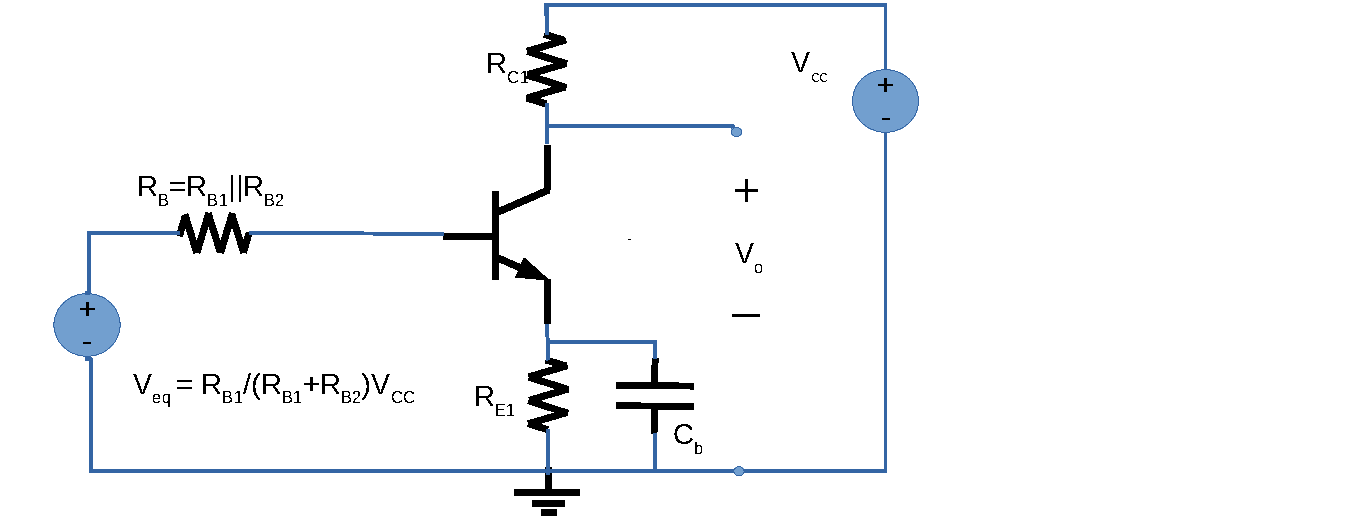
\includegraphics[width=0.8\linewidth]{gainstage.pdf}
\caption{Gain Stage Circuit}                                     %%%%%%%%%%LEGENDA
\label{fig:gscircuit}
\end{figure}


\begin{table}[H]
  \centering
  \begin{tabular}{|l|r|}
     \hline    
    {\bf Name} & {\bf Value} \\ \hline   
    $V_{T}$ & 0.025000 V\\ \hline
$beta$ & 178.700000 \\ \hline
$V_{A}$ & 69.700000 V\\ \hline
$V_{BEON}$ & 0.700000 V \\ \hline

  \end{tabular}
  \caption{BC547A model}
  \label{tab:bgs}
\end{table}

\subsubsection{Operating Point}
Considering the equations of the lecture 17 and the theoretical DC model studied , we compute the OP. The table~\ref{tab:opgs} presents the results obtained.

\begin{table}[H]
  \centering
  \begin{tabular}{|l|r|}
     \hline    
    {\bf Name} & {\bf Value} \\ \hline   
    $R_{B}$ & 1.600000e+04 Ohm\\ \hline
$V_{eq}$ & 2.400000e+00 V\\ \hline
$I_{B1}$ & 1.094885e-05 A \\ \hline
$I_{C1}$ & 1.956559e-03 A \\ \hline
$I_{E1}$ & 1.967508e-03 A \\ \hline
$V_{E1}$ & 1.524818e+00 V \\ \hline
$V_{O1}$ & 1.016083e+01 V \\ \hline
$V_{CE}$ & 8.636016e+00 V \\ \hline

  \end{tabular}
  \caption{OP - Gain Stage}
  \label{tab:opgs}
\end{table}


